% !TeX program = xelatex
% =====================================================================
%  اسلایدهای دفاع پایان‌نامه کارشناسی — دانشگاه بناب
%  روش ساخت: xelatex slides.tex (دو بار)
% =====================================================================
\documentclass[12pt,aspectratio=169]{beamer}

\usetheme{Madrid}
\usefonttheme{professionalfonts}

\usepackage{xepersian}
\settextfont[Path=fonts/,Extension=.ttf,UprightFont=*-Regular,BoldFont=*-Bold,Scale=1.0]{Vazirmatn}
\setlatintextfont[Scale=MatchLowercase]{TeX Gyre Termes}
\DefaultMathsDigits

\setbeamertemplate{navigation symbols}{}
\graphicspath{{figs/}}

\title[شبکه‌های عصبی آگاه از فیزیک]{شبکه‌های عصبی آگاه از فیزیک برای حل مسائل مستقیم و معکوس معادلات دیفرانسیل جزئی غیرخطی}
\author[محمد امیر بابازاد]{محمد امیر بابازاد \\ \small استاد راهنما: دکتر بابک آذرنوید}
\institute[دانشگاه بناب]{دانشگاه بناب، گروه علوم کامپیوتر}
\date{شهریور ۱۴۰۵}
\titlegraphic{
\includegraphics[height=1.6cm]{logo}}

\begin{document}

% ---------- عنوان ----------
\begin{frame}[plain]
\titlepage
\end{frame}

% ---------- فهرست ----------
\begin{frame}{فهرست ارائه}
\tableofcontents
\end{frame}

% ================= مقدمه =================
\section{مقدمه}

\begin{frame}{بیان مسئله}
\begin{itemize}
\item بخش بزرگی از پدیده‌های فیزیکی و مهندسی با معادلات دیفرانسیل جزئی \lr{(PDE)} توصیف می‌شوند.
\item روش‌های عددی کلاسیک (تفاضل محدود، المان محدود، طیفی) به شبکه محاسباتی وابسته‌اند و در ابعاد بالا با نفرین ابعاد مواجه می‌شوند.
\item مدل‌های یادگیری عمیق صرفاً داده‌محور به داده فراوان نیاز دارند و سازگاری آن‌ها با قوانین فیزیک تضمین‌شده نیست.
\item \textbf{پرسش اصلی:} چگونه معادله حاکم بر سیستم را مستقیماً وارد آموزش شبکه عصبی کنیم؟
\item پاسخ: شبکه‌های عصبی آگاه از فیزیک \lr{(PINN)}، معرفی‌شده توسط رئیسی و همکاران (۲۰۱۹).
\end{itemize}
\end{frame}

\begin{frame}{اهداف پژوهش}
\begin{enumerate}
\item مطالعه مبانی: معادلات دیفرانسیل جزئی، روش‌های عددی، شبکه‌های عصبی و مشتق‌گیری خودکار
\item بررسی چارچوب آگاه از فیزیک: مدل‌های زمان‌پیوسته و زمان‌گسسته، مسائل مستقیم و معکوس
\item پیاده‌سازی حل‌گر مرجع مستقل (طیفی فوریه + گام‌زنی نمایی مرتبه چهار)
\item حل مستقیم معادله برگرز تنها با داده اولیه و مرزی
\item کشف ضرایب معادله از روی مشاهده‌های پراکنده و بررسی اثر نویز
\end{enumerate}
\end{frame}

% ================= مبانی =================
\section{مبانی نظری}

\begin{frame}{معادلات دیفرانسیل جزئی و معادله برگرز}
\begin{itemize}
\item صورت کلی:
\begin{equation*}
u_t + \mathcal{N}[u; \lambda] = 0
\end{equation*}
\item مسئله \textbf{مستقیم}: پارامترها معلوم، جواب مجهول است.
\item مسئله \textbf{معکوس}: از روی مشاهده‌ها، پارامترها شناسایی می‌شوند.
\item معادله برگرز (مسئله نمونه این پژوهش):
\begin{equation*}
u_t + u u_x - \nu u_{xx} = 0
\end{equation*}
\item رقابت جمله غیرخطی و جمله پخش، جبهه‌های تندی ایجاد می‌کند که محک استاندارد روش‌های عددی است.
\end{itemize}
\end{frame}

\begin{frame}{روش‌های عددی کلاسیک}
\begin{itemize}
\item \textbf{تفاضل‌های محدود:} تقریب مشتق با نقاط مجاور؛ ساده ولی ناکارآمد در هندسه‌های پیچیده
\item \textbf{المان‌های محدود:} تقسیم دامنه به المان؛ انعطاف بالا ولی پرهزینه
\item \textbf{روش‌های طیفی:} بسط بر حسب توابع پایه سراسری؛ دقت عالی برای جواب‌های هموار
\end{itemize}
\vspace{3mm}
\begin{block}{محدودیت مشترک}
وابستگی به شبکه محاسباتی، اجرای مجدد برای هر شرط جدید، و رشد نمایی هزینه در ابعاد بالا
\end{block}
\end{frame}

\begin{frame}{شبکه‌های عصبی و آموزش}
\begin{itemize}
\item پرسپترون چندلایه: ترکیب توابع خطی و فعال‌سازهای غیرخطی مانند تانژانت هیپربولیک
\item قضیه تقریب جهانی: توانایی تقریب هر تابع پیوسته با دقت دلخواه
\item آموزش = کمینه‌سازی تابع هزینه، معمولاً میانگین مربعات خطا:
\begin{equation*}
\mathrm{MSE} = \frac{1}{N}\sum_{i=1}^{N} (u_\theta(\mathbf{x}_i) - u_i)^2
\end{equation*}
\item بهینه‌سازها: آدام (شروع سریع) و \lr{L-BFGS} (دقت نهایی بالا)
\item گرادیان‌ها با الگوریتم پس‌انتشار محاسبه می‌شوند.
\end{itemize}
\end{frame}

\begin{frame}{مشتق‌گیری خودکار}
\begin{itemize}
\item محاسبه دقیق مشتق (تا دقت ماشین) با اعمال قاعده زنجیره‌ای روی گراف محاسباتی برنامه
\item بدون خطای برشی تفاضل محدود و بدون انفجار عبارت‌های نمادی
\item حالت معکوس: گرادیان یک خروجی نسبت به هزاران پارامتر، با حدود دو برابر هزینه یک اجرا
\item دو نقش کلیدی در این پژوهش:
\begin{enumerate}
\item به‌روزرسانی وزن‌های شبکه در آموزش
\item محاسبه مشتق‌های جواب نسبت به مکان و زمان برای ساخت باقیمانده معادله
\end{enumerate}
\end{itemize}
\end{frame}

% ================= روش =================
\section{روش پژوهش}

\begin{frame}{ایده محوری شبکه آگاه از فیزیک}
\begin{itemize}
\item جواب با شبکه عمیق تقریب زده می‌شود: $u(t,\mathbf{x}) \approx u_\theta(t,\mathbf{x})$
\item مشتق‌ها با مشتق‌گیری خودکار به دست می‌آیند و باقیمانده تعریف می‌شود:
\begin{equation*}
f(t,\mathbf{x}) := u_t + \mathcal{N}[u]
\end{equation*}
\item خود $f$ نیز یک شبکه عصبی است (با همان پارامترها).
\item تابع هزینه ترکیبی:
\begin{equation*}
\mathrm{MSE} = \mathrm{MSE}_u + \mathrm{MSE}_f
\end{equation*}
\item جمله فیزیکی مانند منظم‌ساز عمل می‌کند: دقت بالا با داده اندک!
\end{itemize}
\end{frame}

\begin{frame}{مدل‌های زمان‌پیوسته و زمان‌گسسته}
\begin{block}{مدل زمان‌پیوسته (پیاده‌سازی‌شده در این پژوهش)}
ورودی $(t,\mathbf{x})$ و خروجی $u(t,\mathbf{x})$؛ آموزش با داده اولیه/مرزی و اجبار معادله در نقاط هم‌مکانی
\end{block}
\vspace{2mm}
\begin{block}{مدل زمان‌گسسته (بررسی نظری)}
استفاده از طرح رانگ ـ کوتای ضمنی با $q$ مرحله؛ امکان گام زمانی بسیار بزرگ و پایدار
\end{block}
\vspace{2mm}
\begin{itemize}
\item در مسئله برگرز: $f = u_t + u u_x - \nu u_{xx}$
\end{itemize}
\end{frame}

\begin{frame}{مسئله معکوس: کشف پارامترها}
\begin{itemize}
\item پارامترهای $\lambda$ جزء متغیرهای قابل‌آموزش می‌شوند و همان تابع هزینه نسبت به $(\theta, \lambda)$ کمینه می‌شود.
\item داده‌ها: مشاهده‌های پراکنده در کل دامنه (نه فقط مرز).
\item در مسئله برگرز:
\begin{equation*}
f = u_t + \lambda_1 u u_x - \lambda_2 u_{xx}
\end{equation*}
\item شبکه هم‌زمان جواب را بازسازی و ضرایب را شناسایی می‌کند.
\item مزیت نسبت به روش‌های کتابخانه‌محور: بدون نیاز به جملات کاندید و مقاوم‌تر در برابر نویز.
\end{itemize}
\end{frame}

% ================= پیاده‌سازی =================
\section{پیاده‌سازی و نتایج}

\begin{frame}{محیط پیاده‌سازی و حل‌گر مرجع}
\begin{itemize}
\item پایتون و کتابخانه جکس \lr{(JAX)}؛ آموزش دومرحله‌ای آدام و \lr{L-BFGS}؛ اجرا روی پردازنده مرکزی
\item حل‌گر مرجع مستقل: طیفی فوریه (۱۰۲۴ مود) + گام‌زنی \lr{ETDRK4}
\item راستی‌آزمایی حل‌گر با دو آزمون مستقل:
\begin{enumerate}
\item همگرایی: تغییر $6.2\times 10^{-9}$ با نصف شدن گام زمانی
\item تطابق با جواب نیمه‌تحلیلی کول ـ هوپف تا مرتبه $10^{-8}$ دور از جبهه
\end{enumerate}
\item شبکه مستقیم: ۴ لایه ۵۰ نورونی (۷۸۵۱ پارامتر)؛ ۲۰۰ داده و ۱۰۰۰۰ نقطه هم‌مکانی
\item شبکه معکوس: ۵ لایه ۳۰ نورونی؛ ۵۰۰۰ مشاهده پراکنده
\end{itemize}
\end{frame}

\begin{frame}{نتیجه مسئله مستقیم}
\begin{center}
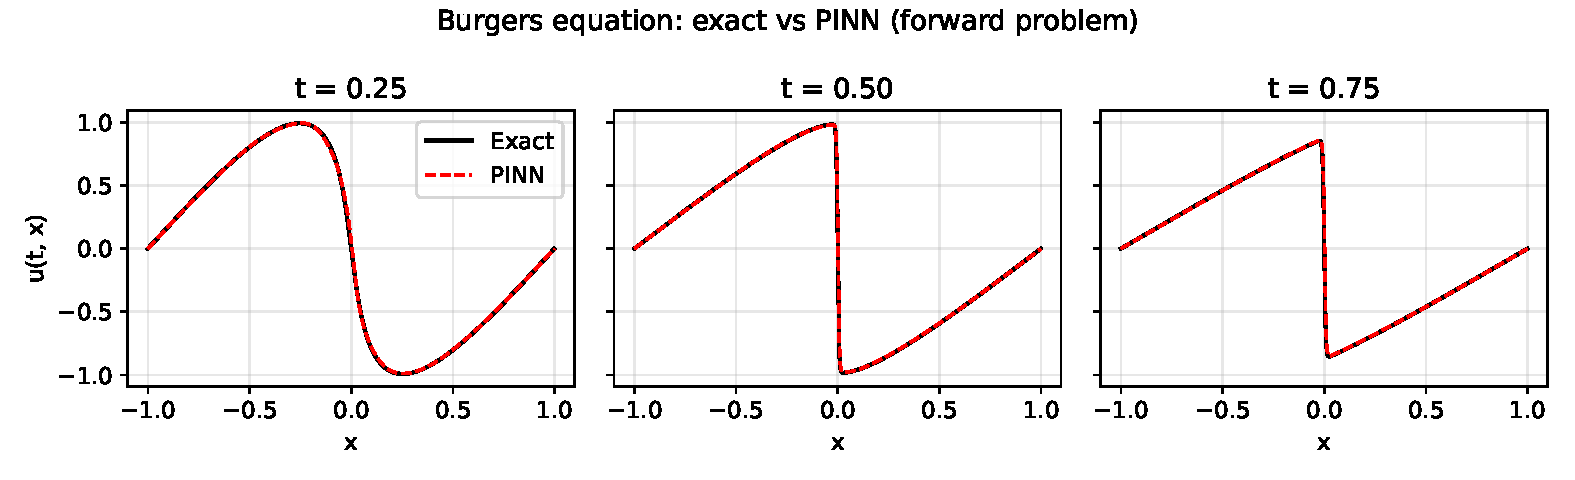
\includegraphics[width=0.95\textwidth]{burgers_snapshots}
\end{center}
\begin{itemize}
\item خطای نسبی $2.15\times 10^{-2}$ تنها با ۲۰۰ نقطه داده اولیه و مرزی
\end{itemize}
\end{frame}

\begin{frame}{توزیع خطا و همگرایی آموزش}
\begin{minipage}{0.48\textwidth}
\centering
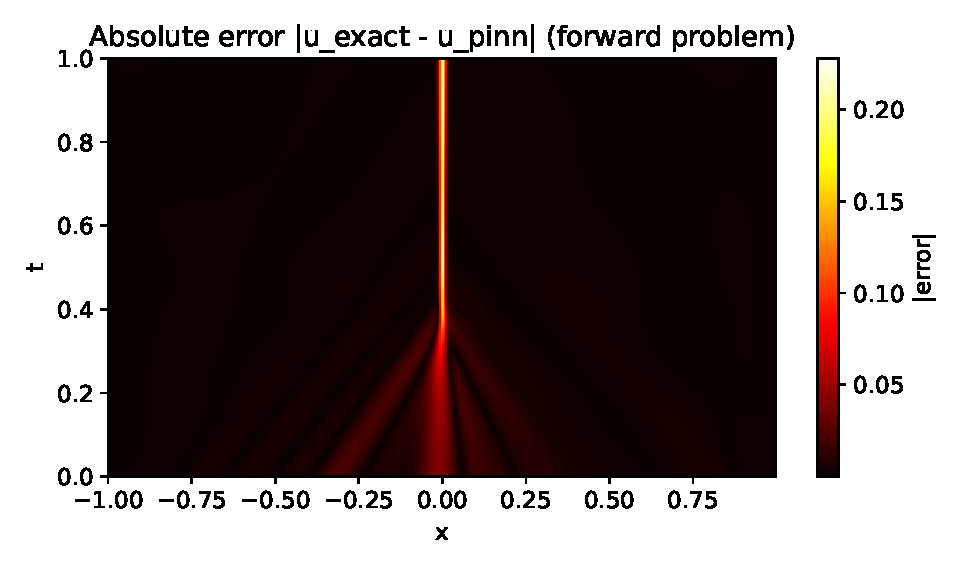
\includegraphics[width=\textwidth]{error_heatmap}
\end{minipage}
\hfill
\begin{minipage}{0.48\textwidth}
\centering
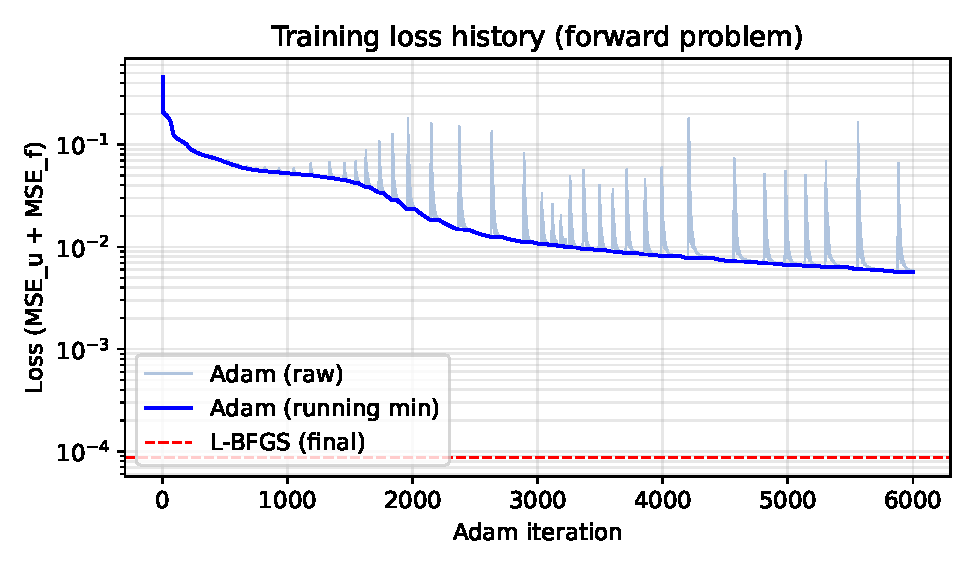
\includegraphics[width=\textwidth]{loss_history}
\end{minipage}
\begin{itemize}
\item خطا فقط در لایه باریک جبهه موج متمرکز است؛ بهبود نهایی با \lr{L-BFGS}
\end{itemize}
\end{frame}

\begin{frame}{نتیجه مسئله معکوس}
\begin{center}
\begin{tabular}{|c|c|c|c|c|}
\hline
\textbf{سناریو} & \textbf{$\lambda_1$} & \textbf{خطا} & \textbf{$\lambda_2$} & \textbf{خطا} \\
\hline
بدون نویز & $0.912$ & $8.8\%$ & $4.22\times 10^{-3}$ & $32.6\%$ \\
\hline
نویز یک درصد & $0.923$ & $7.7\%$ & $3.97\times 10^{-3}$ & $24.9\%$ \\
\hline
مقدار واقعی & \multicolumn{2}{c|}{$1$} & \multicolumn{2}{c|}{$0.00318$} \\
\hline
\end{tabular}
\end{center}
\vspace{2mm}
\begin{itemize}
\item ضریب انتقال با دقت قابل‌قبول و مرتبه بزرگی ضریب پخش به‌درستی شناسایی شد.
\item نویز یک درصد دقت را به‌طور چشمگیری تخریب نکرد (پایداری روش).
\end{itemize}
\end{frame}

\begin{frame}{بحث نتایج}
\begin{itemize}
\item \textbf{کارایی داده‌ای:} بازسازی کل دامنه با ۲۰۰ نقطه در برابر صد هزار نقطه شبکه مرجع
\item \textbf{گلوگاه دقت:} تفکیک لایه تند جبهه؛ تمرکز نقاط هم‌مکانی در این ناحیه مؤثر بود
\item \textbf{حساسیت $\lambda_2$:} کوچکی مقدار و موضعی بودن اثر پخش، شناسایی دقیق را ذاتاً دشوار می‌کند
\item \textbf{مقایسه با مقاله:} بازتولید کیفی کامل رفتار روش با امکانات محدود (پردازنده مرکزی)
\item \textbf{جایگاه روش:} مکمل روش‌های کلاسیک در مسائل معکوس و داده ناقص، نه جایگزین آن‌ها
\end{itemize}
\end{frame}

% ================= جمع‌بندی =================
\section{جمع‌بندی}

\begin{frame}{نتیجه‌گیری}
\begin{itemize}
\item چارچوب آگاه از فیزیک، دانش معادله را با مشتق‌گیری خودکار وارد آموزش شبکه می‌کند.
\item با داده اندک به جواب قابل‌قبول می‌رسد و پارامترهای مجهول را نیز شناسایی می‌کند.
\item در برابر نویز پایدار است و خروجی آن تابعی پیوسته و مشتق‌پذیر است.
\item محدودیت‌ها: هزینه آموزش، دشواری لایه‌های تند، و نبود تضمین نظری همگرایی.
\end{itemize}
\end{frame}

\begin{frame}{کارهای آینده}
\begin{itemize}
\item پیاده‌سازی مدل زمان‌گسسته و مقایسه با مدل زمان‌پیوسته
\item اعمال روش به معادلات دیگر (گرما، شرودینگر، ناویر ـ استوکس)
\item وزن‌دهی تطبیقی تابع هزینه و نمونه‌برداری تطبیقی نقاط هم‌مکانی
\item مطالعه نظام‌مند اثر معماری شبکه و حجم داده
\item ترکیب با روش‌های برآورد عدم قطعیت
\end{itemize}
\end{frame}

\begin{frame}[plain]
\vspace{15mm}
\begin{center}
{\Large سپاس از توجه شما} \\[6mm]
{\large پرسش‌ها و پاسخ‌ها}
\end{center}
\end{frame}

\end{document}
